\documentclass[11pt]{standalone}
\usepackage{amssymb}
\usepackage{amsmath}
\usepackage[no-math]{fontspec}
\usepackage{unicode-math}
\usepackage{libertinus}
\usepackage{pgf,xcolor}
\usepackage{tikz}
\usetikzlibrary{arrows.meta, backgrounds}
\usepackage{pgfplots}
\pgfplotsset{compat=newest}

\definecolor{my_darkgray}{HTML}{484949}
\definecolor{my_lightgray}{HTML}{F3F4F4}
\definecolor{my_darkblue}{HTML}{005A94}
\definecolor{my_lightblue}{HTML}{CCDEE9}
\definecolor{my_yellow}{HTML}{FFEC7F}
\definecolor{my_red}{HTML}{E60000}
\definecolor{my_orange}{HTML}{E87846}

\begin{document}
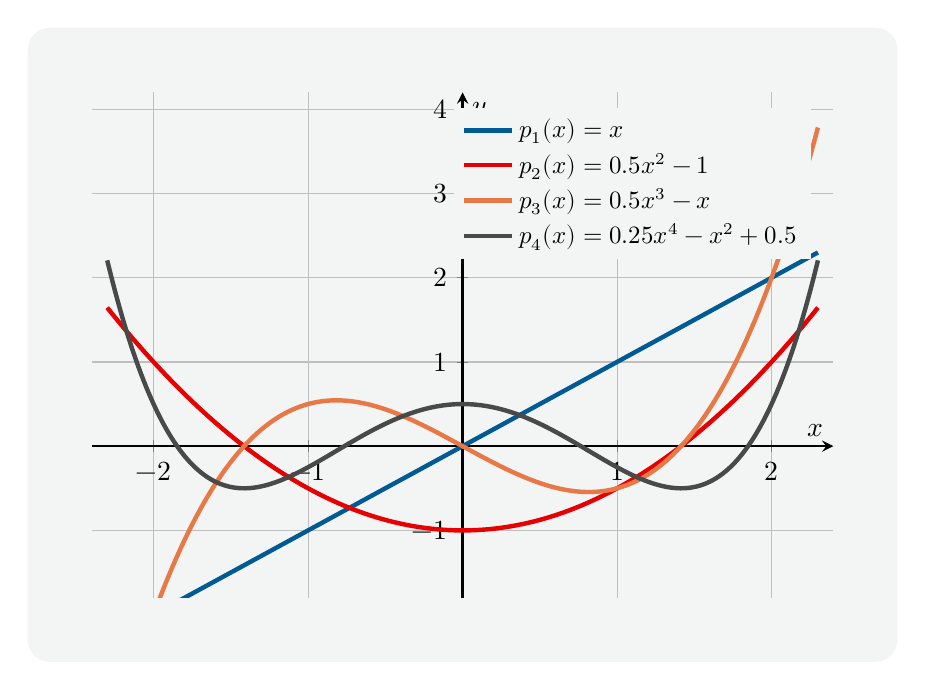
\begin{tikzpicture}[
    show background rectangle,
    background rectangle/.style={fill=my_lightgray, rounded corners=8pt},
    inner frame sep=0.8cm
]
\begin{axis}[
    axis lines=center,
    xlabel={$x$},
    ylabel={$y$},
    height=8cm, width=11cm,
    xmin=-2.4, xmax=2.4,
    ymin=-1.8, ymax=4.2,
    xtick={-2,-1,0,1,2},
    ytick={-1,0,1,2,3,4},
    grid=both,
    axis line style={thick},
    legend style={
        font=\small,
        at={(0.97, 0.97)},
        anchor=north east,
        draw=none,
        fill=my_lightgray,
    },
    legend cell align=left,
    % Clip curves to the axis window
    clip=true,
]

% Polynomials are chosen to show the characteristic shape of each degree
% clearly within the same window and at comparable scales.

% Degree 1 (linear): straight line through origin. Odd function.
% p_1(x) = x
\addplot[draw=my_darkblue, samples=300, ultra thick, domain=-2.3:2.3]{x};
\addlegendentry{$p_1(x)=x$}

% Degree 2 (quadratic): upward parabola with vertex below the x-axis.
% p_2(x) = 0.5x^2 - 1  (vertex at (0,-1), zeros at +/-sqrt(2) ~= +/-1.41)
\addplot[draw=my_red, samples=300, ultra thick, domain=-2.3:2.3]{0.5*x^2 - 1};
\addlegendentry{$p_2(x)=0.5x^2-1$}

% Degree 3 (cubic): S-shaped curve through the origin. Odd function.
% p_3(x) = 0.5x^3 - x  (zeros at 0, +/-sqrt(2); local extrema at +/-sqrt(2/3))
\addplot[draw=my_orange, samples=300, ultra thick, domain=-2.3:2.3]{0.5*x^3 - x};
\addlegendentry{$p_3(x)=0.5x^3-x$}

% Degree 4 (quartic): W-shape. Even function.
% p_4(x) = 0.25x^4 - x^2 + 0.5
%   (global minima at x = +/-sqrt(2) ~= +/-1.41 with value -0.5;
%    local maximum at x=0 with value 0.5)
% my_darkgray is used as the fourth color since the palette provides
% three curve colors (darkblue, red, orange) for three-color figures.
\addplot[draw=my_darkgray, samples=300, ultra thick, domain=-2.3:2.3]
    {0.25*x^4 - x^2 + 0.5};
\addlegendentry{$p_4(x)=0.25x^4-x^2+0.5$}

\end{axis}
\end{tikzpicture}
\end{document}
